\chapter{Arquitectura de Adquisición de Datos y Caracterización de Encoders}

\lineaLateral
\begin{resumenCapitulo}
	En este capítulo se describe la metodología empleada para garantizar una lectura fidedigna de la posición del brazo robótico, abordando desde la integridad física de las señales hasta la estructura de software para el procesamiento de datos.
\end{resumenCapitulo}

\section{Lista de materiales}
\begin{itemize}
	\item Arduino UNO.
	\item Motores del brazo robótico (Mitsubishi Movemaster EX).
	\item Encoders de los motores.
	\item LabVIEW.
	\item Multímetro FLUKE.
	\item Osciloscopio RIGOL DS1202 (2 canales).
\end{itemize}


\section{Identificación y Caracterización de los Módulos de Encoders}

Dada la obsolescencia tecnológica del brazo \textit{Mitsubishi RV-M1} y la carencia de manuales detallados, se ejecutó una fase de inspección física intrusiva en las unidades de captación. Este procedimiento consistió en el desmontaje de las carcasas de los servomotores para acceder a las tarjetas de circuito impreso (PCB) de los encoders ópticos. El objetivo primordial fue validar la correspondencia entre el código de colores del cableado original y los terminales lógicos de cada articulación.

Para mitigar riesgos de cortocircuito o errores de polaridad durante la integración con el microcontrolador, se realizó un rastreo de continuidad desde el extremo del segmento de captación hasta el SDP. Se identificó una arquitectura de señales basada en la siguiente nomenclatura técnica:

\begin{itemize}
	\item \textbf{Canales A / B:} Señales digitales en cuadratura (desfasadas 90°) empleadas para determinar la posición incremental y el sentido de giro.
	\item \textbf{Canal Z (Índice):} Pulso de referencia generado una vez por revolución completa, utilizado para la sincronización del punto de origen (\textit{home}).
	\item \textbf{G (GND) / V (VCC):} Líneas de referencia de tierra y alimentación de voltaje lógico, respectivamente.
\end{itemize}

La inspección hecha en el capítulo pasado permitió identificar variaciones en la resolución nativa de los sensores según el eje. Como se aprecia en la Figura \ref{fig:base_encoder}, la base utiliza una configuración específica, mientras que los ejes de mayor torque (cadera, hombro y codo) comparten el módulo \textbf{Sharp GP1R112} de 200 pasos (ver Figura \ref{fig:encoderm2m3}). Por el contrario, las articulaciones finales (antebrazo y muñeca) emplean una variante de menor resolución, con 96 pasos, detallada en la Figura \ref{fig:m4m5_encoder}.


\begin{figure}[htbp]
	\centering
	
\includegraphics[width=0.5\linewidth]{images/encoders/screenshot002}
	\caption[Módulo de captación: Eje de la Base]{Módulo de captación ubicado en la base del brazo robótico.}
	\label{fig:base_encoder}
\end{figure}

\begin{figure}[htbp]
	\centering
	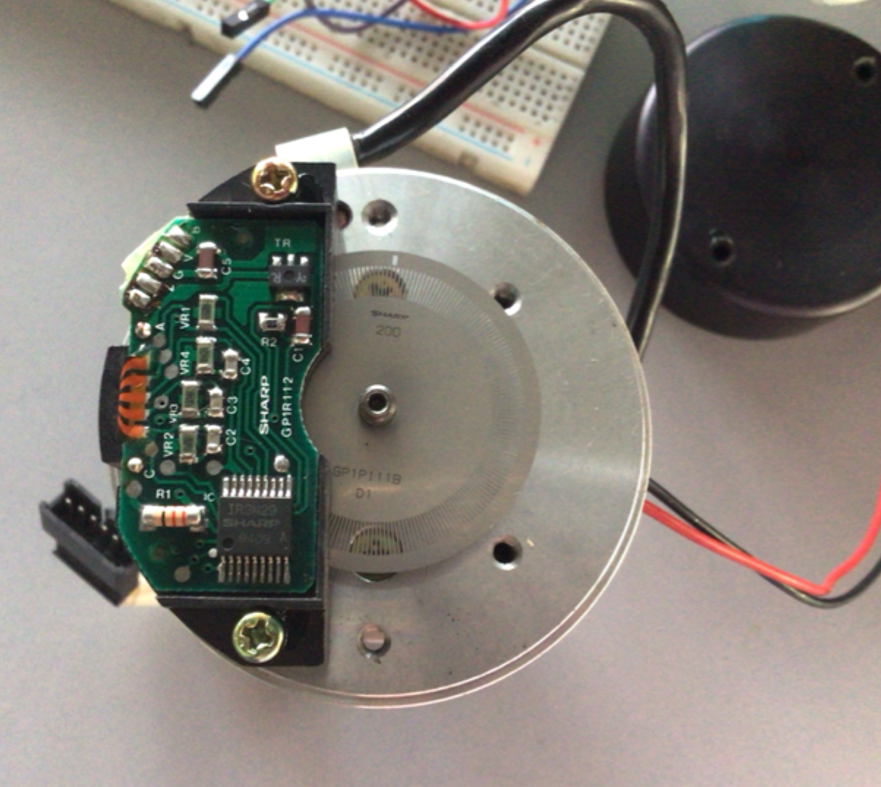
\includegraphics[width=0.6\linewidth]{images/encoders/encoderm2m3}
	\caption[Sensor Sharp GP1R112: Ejes M2 y M3]{Sensor de cuadratura Sharp GP1R112 (200 PPR) integrado en las articulaciones M2 y M3.}
	\label{fig:encoderm2m3}
\end{figure}

\begin{figure}[htbp]
	\centering
	
\includegraphics[width=0.5\linewidth]{images/encoders/screenshot001}
	\caption[Sensor Sharp GP1R112: Ejes M4 y M5]{Variante del sensor Sharp GP1R112 (96 PPR) para los ejes terminales M4 y M5.}
	\label{fig:m4m5_encoder}
\end{figure}


\clearpage
\subsection{Determinación de la Resolución de los Encoders}

Para establecer la resolución base del sistema de retroalimentación, se procedió a la apertura mecánica de las carcasas de los actuadores, permitiendo el acceso directo a los discos ópticos de los encoders (fig. \ref{fig:disco_encoder}). Se identificó el uso de tecnología de interrupción óptica mediante discos metálicos ranurados; este mecanismo opera permitiendo o bloqueando el paso de un haz de luz infrarroja hacia un fototransistor, generando así los pulsos digitales que el microcontrolador contabiliza como pasos de movimiento.

\begin{figure}[htbp]
	\centering
	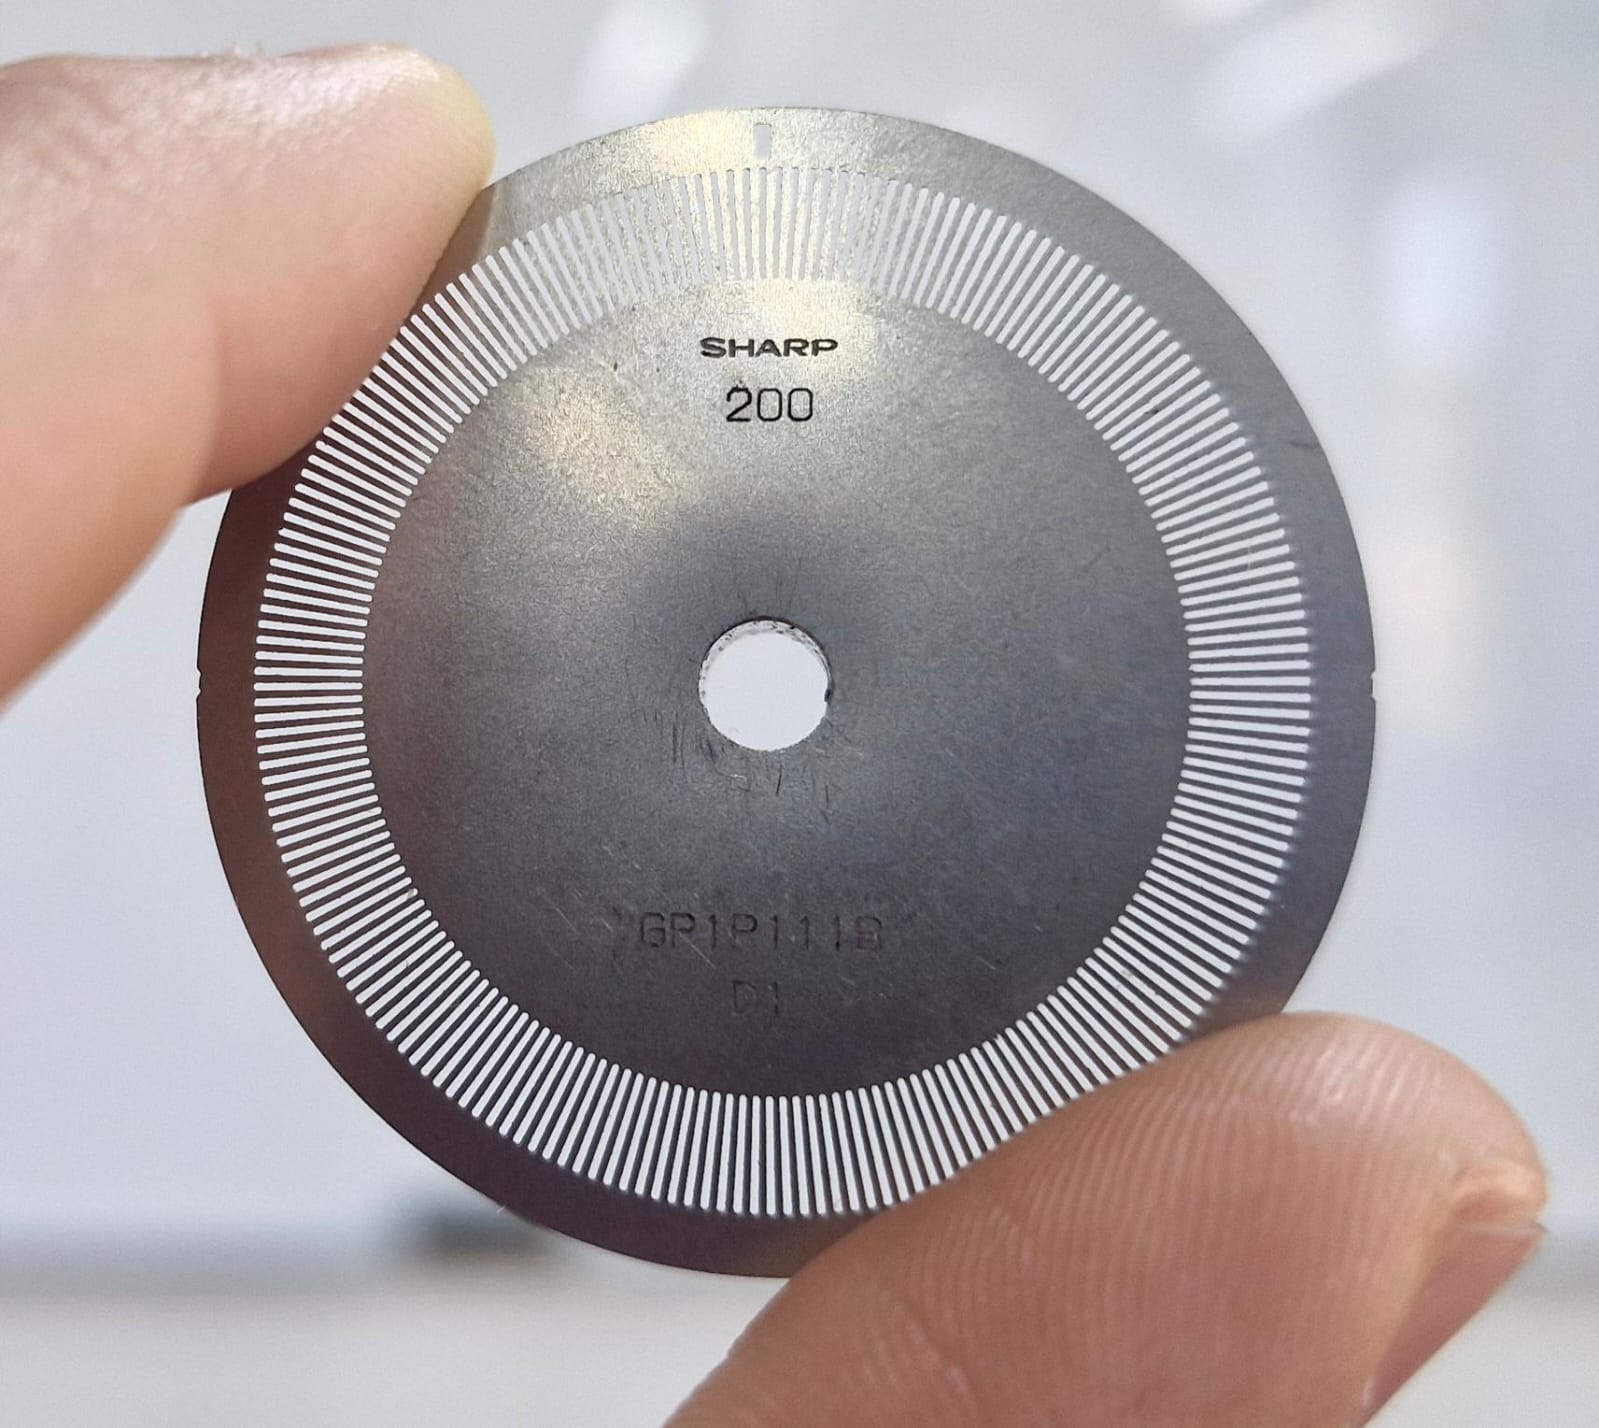
\includegraphics[width=0.5\linewidth]{images/encoders/disco.png}
	\caption[Disco óptico del encoder Sharp]{Disco metálico ranurado ubicado en el encoder de la cadera. Tiene una resolución de 200 pasos.}
	\label{fig:disco_encoder}
\end{figure}

Como se observa en la evidencia física del modelo \textbf{SHARP GP1R112}, el disco cuenta con una serie de ranuras equidistantes que definen su resolución nativa. No obstante, se partió de la premisa de que la resolución (pasos por revolución) no es uniforme en todos los ejes del brazo, debido a las distintas relaciones de transmisión mecánica de cada articulación. Esta hipótesis fue confirmada posteriormente mediante el análisis de frecuencia en osciloscopio, cuyos resultados se contrastan con el mapeo de señales detallado en las tablas \ref{tab:encoder_cadera} a la \ref{tab:encoder_muneca}.

\section{Conexión de los Encoders}

Dado que los encoders del \textit{Mitsubishi RV-M1} operan bajo una configuración de colector abierto, el sistema no entrega un nivel de voltaje alto por sí mismo, sino que requiere una red de polarización externa para definir los estados lógicos. Para corroborar este comportamiento y asegurar la integridad de las señales antes de su integración con el microcontrolador, se procedió a realizar una validación en tres etapas: modelado, simulación y experimentación física.

En primera instancia, se replicó la etapa de salida del encoder en \textit{Proteus} utilizando transistores de unión bipolar para emular el corte y saturación del colector. Como se observa en la Figura \ref{fig:esquema_encoder_oc}, la adición de una resistencia de \textit{pull-up} de $1k\Omega$ permitió obtener una oscilación de $0V$ a $5V$, confirmando que esta impedancia es suficiente para saturar el nodo sin comprometer la velocidad de conmutación. 

Posteriormente, se trasladó el diseño a una implementation física (ver Figura \ref{fig:conexioncables}). Se identificó el orden de los conductores respetando la secuencia de señales: Index (Z), Canal A, Canal B, GND y VCC. La respuesta dinámica capturada en el osciloscopio (Figura \ref{fig:osc_pullup_test}) muestra una señal cuadrada limpia y libre de ruido significativo, validando que el arreglo de resistencias es el adecuado para garantizar lecturas estables en los contadores de alta velocidad del sistema de control.

\begin{figure}[p] 
	\centering
	
	% --- FILA SUPERIOR ---
	\begin{minipage}{0.48\textwidth}
		\centering
		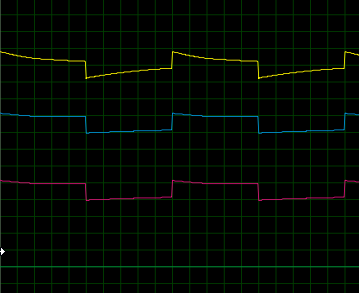
\includegraphics[width=\linewidth]{images/encoders/senalosci.png}
		\caption[Validación dinámica en osciloscopio]{\small Validación dinámica: Señal cuadrada obtenida en el osciloscopio.}
		\label{fig:osc_pullup_test}
	\end{minipage}
	\hfill
	\begin{minipage}{0.48\textwidth}
		\centering
		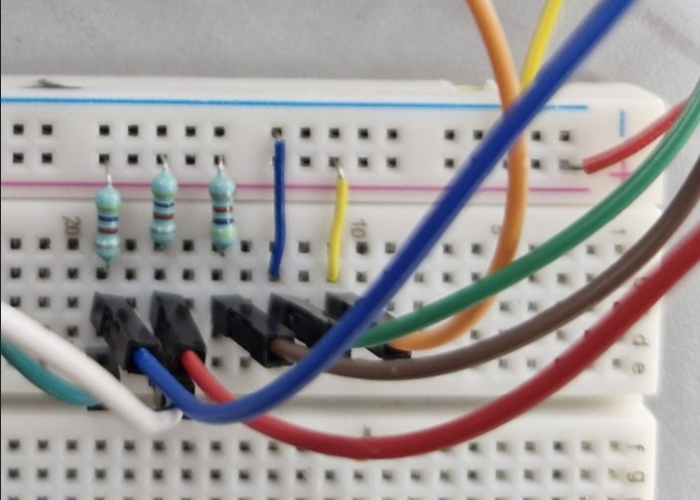
\includegraphics[width=\linewidth]{images/encoders/conexionCables}
		\caption[Implementación física de resistencias]{\small Implementación física: Arreglo de resistencias y cableado.}
		\label{fig:conexioncables}
	\end{minipage}
	
	\vspace{1cm} 
	
	% --- FILA INFERIOR (AHORA CON DOS IMÁGENES) ---
	\begin{minipage}{0.48\textwidth}
		\centering
		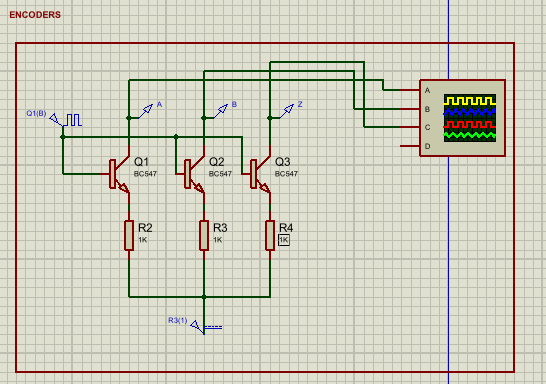
\includegraphics[width=\linewidth]{images/encoders/encodersProteus.png}
		\caption[Modelado técnico en Proteus]{\small \textbf{Modelado en Proteus:} Diseño del circuito de acondicionamiento para encoders.}
		\label{fig:esquema_encoder_oc}
	\end{minipage}
	\hfill
	\begin{minipage}{0.48\textwidth}
		\centering
		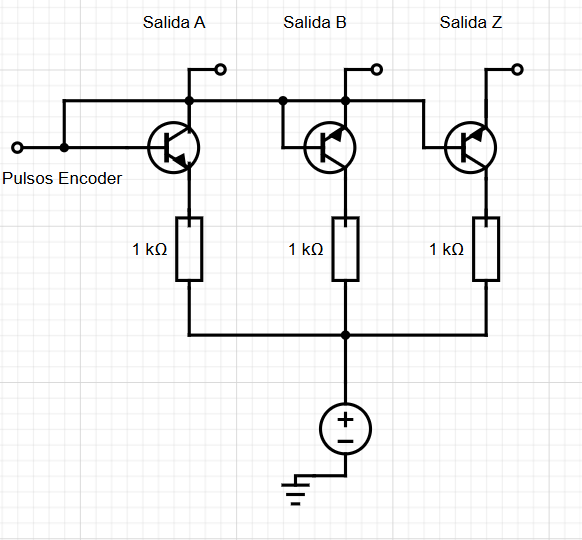
\includegraphics[width=\linewidth]{images/encoders/diagramaelectrico}
		\caption[Diagrama de conexión física]{\small \textbf{Conexión del Sistema:} Se representa el funcionamiento del sensor en su aplicación de colector abierto y las resistencias físicas colocadas a 5V.}
		\label{fig:diagramaelectrico}
	\end{minipage}
	
	\vspace{0.8cm}
	{\small \centering Análisis comparativo entre la respuesta experimental y el modelo circuital propuesto para la etapa de retroalimentación.\par}
\end{figure}
\clearpage

\subsection{Validación de Resolución y Diagnóstico mediante Canal Z y Osciloscopio}

Tras la inspección física de los discos ranurados, fue imperativo verificar la integridad funcional de los fototransistores y el estado mecánico de las rendijas. Dado el tiempo de operación del brazo \textit{Mitsubishi RV-M1}, existe el riesgo de obstrucciones por partículas o degradación de la señal óptica, lo que provocaría una lectura errática de la posición.

Para ello, se implementó una metodología de diagnóstico mediante osciloscopio, utilizando el \textbf{Canal Z (Índice)} como gatillo (\textit{trigger}) de referencia. Esta señal, que genera un pulso único por cada 360° de giro, permitió asegurar que se completara una revolución exacta para contabilizar los pulsos del \textbf{Canal A}. Esta técnica de ventaneo electrónico es el único método fiable para confirmar si la resolución física del disco coincide con la señal procesada por el sistema.

Asimismo, se somete al conjunto motor-encoder a una prueba de esfuerzo alimentando el actuador a \textbf{12V}, lo cual representa el límite superior de operación de la etapa de potencia diseñada para este proyecto. El objetivo de esta prueba en condiciones límite fue:
\begin{itemize}
	\item \textbf{Detección de pérdida de pasos:} Verificar si a máxima velocidad angular el sensor es capaz de mantener la frecuencia de conmutación sin omitir pulsos.
	\item \textbf{Validación de la respuesta dinámica:} Confirmar que la resolución se mantiene constante incluso en los picos de torque del motor.
\end{itemize}

Este proceso de caracterización garantizó que los datos registrados en las tablas \ref{tab:encoder_cadera} a la \ref{tab:encoder_muneca} no solo representan el diseño teórico, sino la capacidad real de respuesta del hardware.

% --- ENCODER 2 ---
\begin{figure}[htbp]
	\centering
	\includegraphics[width=0.85\linewidth]{images/encoders/qp5}
	\caption[Validación Encoder 2]{Validación de resolución del \textbf{Encoder 2 (Hombro)}: 200 PPR.}
	\label{fig:ds1zquickprint5}
\end{figure}

% --- ENCODER 3 ---
\begin{figure}[htbp]
	\centering
	\includegraphics[width=0.85\linewidth]{images/encoders/qp2}
	\caption[Validación Encoder 3]{Validación de resolución del \textbf{Encoder 3 (Codo)}: 200 PPR.}
	\label{fig:ds1zquickprint2}
\end{figure}

% --- ENCODER 4 ---
\begin{figure}[htbp]
	\centering
	
\includegraphics[width=0.85\linewidth]{images/encoders/screenshot003}
	\caption[Validación Encoder 4]{Validación de resolución del \textbf{Encoder 4 (Antebrazo)}: 96 PPR.}
	\label{fig:screenshot003a}
\end{figure}

% --- ENCODER 5 ---
\begin{figure}[htbp]
	\centering
	\includegraphics[width=0.85\linewidth]{images/encoders/qp8}
	\caption[Validación Encoder 5]{Validación de resolución del \textbf{Encoder 5 (Muñeca)}: 96 PPR.}
	\label{fig:ds1zquickprint8}
\end{figure}

% --- TABLA DE RESUMEN ---
\begin{table}[htbp]
	\centering
	\caption[Resumen de caracterización técnica]{Resumen de caracterización técnica y validación de resolución por eje.}
	\label{tab:validacion_encoders}
	\renewcommand{\arraystretch}{1.5}
	\rowcolors{2}{green!5}{white}
	\begin{tabular}{lllc}
		\toprule
		\rowcolor{green!15} \textbf{ID} & \textbf{Ubicación} & \textbf{Modelo Sensor} & \textbf{Resolución (PPR)} \\ 
		\midrule
		Encoder 1   & Base                & GP1R112                & 200\\
		Encoder 2   & Hombro              & GP1R112                & 200                       \\
		Encoder 3   & Codo                & GP1R112                & 200                       \\
		Encoder 4   & Antebrazo (M4)      & GP1R112                & 96                        \\
		Encoder 5   & Muñeca (M5)         & GP1R112                & 96                        \\
		\bottomrule
	\end{tabular}
\end{table}

\section{Implementación Inicial con Arduino y Limitaciones Técnicas}
La primera fase consistió en usar un Arduino (Atmega328P) con interrupciones externas. Sin embargo, se identificaron limitantes críticas:
\begin{itemize}
	\item \textbf{Saturación del CPU:} El procesador se dedicaba casi exclusivamente a atender las interrupciones de los 6 ejes.
	\item \textbf{Pérdida de Pulsos:} La arquitectura de un solo hilo causó pérdida de pasos en altas velocidades.
	\item \textbf{Umbrales TTL:} Los 3.3V de los encoders operaban muy cerca del límite de incertidumbre del Arduino de 5V.
\end{itemize}
Por ello, se optó por una estrategia de \textbf{muestreo determinístico} que garantiza la captura de cada flanco sin pérdida de pasos. El siguiente pseudocódigo describe la arquitectura del programa, dividiendo las tareas críticas (dentro de la interrupción) de las tareas de gestión (en el ciclo principal).

\subsection{Procesamiento de Encoders y Optimización por Hardware}

Para la lectura de los encoders, se descartó el uso de interrupciones externas convencionales (\textit{External Interrupts}), ya que la alta frecuencia de pulsos generada por los cinco motores simultáneamente saturaba el procesador, provocando un comportamiento errático en el giro de los motores y pérdida de pasos. 

En su lugar, se implementó una estrategia de \textbf{muestreo por interrupción de temporizador (Timer Interrupt Handling)} utilizando el Timer 5 del ATMega2560.

\subsubsection{Configuración del Timer 5 y Resolución de Pasos}
El Timer 5 se configuró en modo CTC (\textit{Clear Timer on Compare Match}) con un valor de comparación de 199 y un prescaler de 8. Esto genera una frecuencia de muestreo de 10 kHz (cada 100 $\mu$s). Esta frecuencia es lo suficientemente alta para capturar todos los cambios de fase sin sobrecargar la CPU, permitiendo que el hilo principal del programa ejecute la lógica de control y comunicación sin retardos.

En cuanto a la resolución, se implementó una decodificación de tipo \textbf{Half-Quad}. Aunque el disco físico del encoder del Mitsubishi Move Master EX posee 200 ranuras, la lógica de software permite detectar cambios de estado específicos que duplican la resolución efectiva a 400 pasos por revolución, logrando un equilibrio ideal entre precisión posicional y carga computacional.

\subsubsection{Algoritmo de Tabla de Búsqueda (Look-up Table)}
Para determinar el sentido de giro y el conteo de pasos de forma ultra rápida dentro de la ISR (\textit{Interrupt Service Routine}), se utilizó una tabla de estados precalculada:

\begin{lstlisting}[language=C++, caption={Tabla de estados para decodificacion de Encoders}, label={lst:encoder_table}]
	const int8_t encoderTable[16] = {
		0, 0, 0, 0,   // Sin cambio o estados invalidos
		1, 0, 0, -1,  // Incremento detectado / Error
		-1, 0, 0, 1,   // Decremento detectado / Error
		0, 0, 0, 0    // Sin cambio o estados invalidos
	};
\end{lstlisting}

La lógica consiste en concatenar el estado anterior de las fases A y B con el estado actual, formando un índice de 4 bits (valores de 0 a 15). Este índice accede directamente a la tabla, la cual devuelve un \textbf{1} para incrementar, un \textbf{-1} para decrementar o un \textbf{0} si no hubo cambio o si el cambio detectado es físicamente imposible (ruido).

\subsubsection{Pseudocódigo de la Lógica de Lectura}
El siguiente pseudocódigo ilustra la operación realizada cada 100 microsegundos:

\begin{center}
	\begin{minipage}{0.8\textwidth}
		\begin{tcolorbox}[colback=green!5, colframe=green!30!black, title=Algoritmo de Muestreo (ISR Timer 5)]
			\small
			\begin{enumerate}
				\item \textbf{Para cada} motor $i$ del 0 al 4:
				\begin{enumerate}
					\item Leer estados físicos de los pines Fase A y Fase B.
					\item Combinar estados: $Actual = (FaseA \ll 1) \text{ OR } FaseB$.
					\item Crear índice: $Indice = (Anterior[i] \ll 2) \text{ OR } Actual$.
					\item Consultar tabla: $Delta = encoderTable[Indice]$.
					\item Actualizar posición: $Pasos[i] = Pasos[i] + Delta$.
					\item Guardar estado para el siguiente ciclo: $Anterior[i] = Actual$.
				\end{enumerate}
				\item \textbf{Fin del ciclo}
			\end{enumerate}
		\end{tcolorbox}
	\end{minipage}
\end{center}

\begin{lstlisting}[language=C++, caption={Rutina de interrupción para la decodificación de encoders (Timer 5)}, label={lst:isr_encoders}]
	// --- LÓGICA DE ENCODERS (TIMER 5) ---
	// Se ejecuta periódicamente para muestrear las fases A y B
	ISR(TIMER5_COMPA_vect) {
		for (uint8_t i = 0; i < NUM_ENCODERS; i++) {
			// Lectura directa de los registros de puerto para máxima velocidad
			uint8_t a = (*(encoderHw[i].portA) & encoderHw[i].maskA) ? 1 : 0;
			uint8_t b = (*(encoderHw[i].portB) & encoderHw[i].maskB) ? 1 : 0;
			
			// Formación del estado actual (Concatenación de bits)
			uint8_t estadoActual = (a << 1) | b;
			
			// Actualización de la posición usando la tabla de verdad de cuadratura
			// Se compara el estado anterior con el actual para determinar el sentido
			ArrayMotores[i].pasosActuales += encoderTable[(encoderLastState[i] << 2) | estadoActual];
			
			// Preservar el estado para la siguiente iteración
			encoderLastState[i] = estadoActual;
		}
	}
\end{lstlisting}

\begin{resultadosFase}
	Al finalizar el desarrollo de la arquitectura de adquisición y la caracterización de los sistemas de retroalimentación, se consolidaron los siguientes resultados técnicos:
	
	\begin{itemize}
		\item \textbf{Certeza en la Resolución Nativa:} Mediante inspección física y validación con osciloscopio (Trigger en Canal Z), se determinó con precisión la resolución de cada eje, corrigiendo la falta de documentación técnica original. Se validaron 200 PPR para los ejes de alto torque (Base, Hombro, Codo) y 96 PPR para los terminales (Antebrazo, Muñeca).
		
		\item \textbf{Acondicionamiento de Señal Robusto:} Se diseñó e implementó con éxito la red de polarización (\textit{pull-up}) para los encoders de colector abierto, logrando señales cuadradas TTL limpias que garantizan la integridad de los datos ante el ruido electromagnético de los motores.
		
		\item \textbf{Estabilidad y Repetibilidad:} Las pruebas de campo confirmaron que el sistema mantiene el conteo de pasos tras múltiples ciclos de movimiento, limitando los errores únicamente a la inercia mecánica durante la búsqueda de \textit{Home}.
	\end{itemize}
\end{resultadosFase}